\documentclass[a4j]{jarticle}
\usepackage{hetero}
\usepackage{amsmath}
\usepackage{bm}   
\usepackage{graphicx}
\usepackage{url}

%\usepackage[dvips]{graphicx}
%\usepackage{latexsym}

\def\Underline{\setbox0\hbox\bgroup\let\\\endUnderline}
\def\endUnderline{\vphantom{y}\egroup\smash{\underline{\box0}}\\}
\def\|{\verb|} 

%%%%%%%%%%%%%%%%%%%%%%%%%%%%%%%%%%%%%%%%%%%%%%%%%%%%%%%%%%%%%%%%

%\usepackage{listings,jlisting}
\usepackage{listings}
\newcommand{\myvec}[1]{\vec{#1}}
\newcommand{\araa}{Annual Review of Astronomy and Astrophysics}
\newcommand{\icarus}{Icarus}
\newcommand{\mnras}{Monthly Notices of the Royal Astronomical Society}
\newcommand{\apj}{Astrophysical Journal}
\newcommand{\pasa}{Publications of the Astronomical Society of Australia}
\newcommand{\pasj}{Publications of the Astronomical Society of Japan}
\newcommand{\aap}{Astronomy and Astrophysics}
%%%%%%%%%%%%%%%%%%%%%%%%%%%%%%%%%%%%%%%%%%%%%%%%%%%%%%%%%%%%%%%%


  

\title{FDPSによる大規模並列粒子系シミュレーションの \\PEZY-SC2 への実装と性能評価}
  
\etitle{} 

\author{\begin{tabular}{cl}
&岩澤 全規,神戸大学 \\
& 行方大輔,理研R-CCS \\
&野村昴太郎,神戸大学 \\
    & 牧野 淳一郎,神戸大学/理研R-CCS \\
\end{tabular} }

\eauthor{}
\abstract{
粒子法を用いたシミュレーションは科学や工学の幅広い分野で広く使われてお
り、使用されるアルゴリズムも似ている。しかし、今までのソフトウェアは各
分野で独立に開発されており、分野間で共用する事は難しかった。一方、「京」
の様な大規模並列型スパコンで効率よく動作する粒子法プログラムの開発は容
易ではなく、多くの研究者はソフトウェアの開発に多大な時間と労力を割いて
いる。我々は、大規模並列型スパコンで効率よく動
作する粒子法シミュレーションプログラムをユーザーが容易に開発できるフレー
ムワーク(FDPS: Framework for DevelopingParticle Simulator)を開発してい
る。本報告では、PEZY-SC2 上に FDPS をコアとする惑星リングシミュレーショ
ンプログラムを実装し、性能評価をした結果を報告する。
PEZY-SC2 だけでなく、類似したヘテロジニアスメニーコアアーキテクチャをもつ
SW26010 を採用した Sunway Taihuloght での実装と性能についても合わせて
報告する。どちらのアーキテク
チャでも、理論ピークの 35-40\%という高い効率を実現できた。これらのシステムは独自のプログラミング環境の利用を必要とし、また、
アーキテクチャに合わせたチューニングを必要とするため、個々のアプリケー
ション開発者がそのノウハウを獲得し、高い性能を実現することは容易である
とはいいがたいが、フレームワークを利用することで特定マシン向けのチュー
ニングの必要性を減らしていくことが可能となる。
}


\begin{document}

\maketitle



\section{はじめに}

粒子法とは研究対象となる系を相互作用する多数の粒子によって表現し、個々
の粒子の発展方程式を解くことで系の進化をシミュレートする方法である。粒
子法では対象の系の運動に合わせて、自動的に粒子が移動し、系を自然な形で
表現してくれる。そのため、物体の衝突や破壊等、形状が大きく変わる系のシ
ミュレーションや密度コントラストが高い系のシミュレーション等に適してお
り、例えば天文学や生命科学、気象学、防災やものづくりに至るまで幅広い分
野で使われている。

近年、シミュレーションの解像度や精度を上げるために、大規模並列計算機を
使われ始めているが、このような並列計算機上で効率よく動作する、粒子法シ
ミュレーションプログラムを開発する事は容易ではない。効率の良いアプリケー
ション・プログラムを開発するためには、プログラマは各プロセスのロードバ
ランスが取れるように計算領域の分割を行う必要があり、シミュレーション対
象の系が動的に変化していく場合、計算領域を動的に決定する必要がある。

また、計算領域が分割されているので、各プロセスが粒子への相互作用を計算
するためには他のプロセスから相互作用計算に必要となる粒子の情報を受け取る
必要があり、プログラマはこの通信量が最小になる様にソフトウェア開発を行
わなければならない
\cite{WarrenSalmon1992,Makino2004,Springeletal2000,Ishiyamaetal2009b}
。更に、効率的な相互作用の計算のためにはキャッシュメモリやSIMDユニット
の効率的な利用も考慮する必要がある
\cite{2006NewA...12..169N,2012NewA...17...82T,2013NewA...19...74T}。近
年では、相互作用計算を加速するためにGPGPUやその他の加速機も使われ始めて
おり、対応が必要となる場合もある。
\cite{Hamadaetal2009a,Hamadaetal2009b,Bedorf:2014:PGT:2683593.2683600}
 
効率的に動作するプログラムを開発するためには、上記の事柄を考慮する必要
があり、コード開発だけで数年かかってしまうような大規模なプロジェクトに
なってしまう事がある。現状では、コード開発に膨大な時間がかかる事が計算科学全体の
進歩を妨げている。


そこで、我々は上記の問題を解決するためにFDPS(Framework for Developing
Particle Simulator)の開発を行った。FDPSの目的はユーザーが大規模並列計
算機で効率的に動作するプログラムを容易に開発できるようなソフトウェアフ
レームワークを提供する事である。FDPSの基本的な考え方は、粒子法シミュレー
ションプログラムを開発するときに困難となる部分(例えば、領域分割や粒子
交換、効率的な相互作用計算のための粒子の木構造管理等)をFDPS側が担当す
ることである。このため、ユーザーはこの困難な部分を意識することなく、プ
ログラムできる。

ユーザーは相互作用関数と粒子のデータ構造を定義しFDPSに与える事で任意の
2粒子間相互作用を扱うことができる。このため、ユーザーはFDPSを用いて多
くのアプリケションプログラム(例えば、重力N体コード、SPHやMPS等の流体コー
ド、分子動力学コード、個別要素法等)を開発することができる。多粒子間相
互作用に関してはユーザープログラムで対応することができる。

FDPSと同様のコンセプトを持つソフトウェアは幾つか存在するが、それらは相
互作用が$1/r$ポテンシャルのみや\cite{1995CoPhC..87..266W}、密度変化の
大きな系では扱えないなど\cite{Leisheng823}、適用範囲が限定的であり、
FDPSの様な汎用性は備えていない。また、アプリケーション・プログラムの性
能についても非常に高い性能が出る事を確認した。この汎用性の高さと性能の
高さの両立がFDPSの独自性である。

FDPS のようなフレームワークを使うことの意義として、新しいアーキテクチャ
向けの改良やチューニング作業をアプリケーション毎に行う必要がなくなる、
ということがあげられる。これは、本研究の目標であるヘテロジニアス
メニーコアアーキテクチャ上のアプリケーション開発にとっては極めて重要
なことである。フレームワークの内部実装だけを個々のアーキテ
クチャ向けのものに差替えることで、アプリケーションコードは変更なしで
新しいアーキテクチャで高い性能をだす、というのがこのようなフレームワー
クの理想として目指すべきところと考えられる。

本報告では、この理想にいたる途中経過として、 PEZY-SC2 および
Sunway Taihulight での FDPS をベースとした自己重力粒子系計算コードの実
装と性能評価、今後の課題について報告する。

本論文では、FDPSの概要を2節で述べ、
3節では粒子系コード実装の観点からの PEZY-SC2 と Sunway Taihulight アー
キテクチャの特徴をまとめる。4節ではベースとなった FDPS実装からの
変更点についてまとめ、5節で実現した性能、6節で今後の展望についてのべる。

本報告の第一および第二節は情報処理学会研究報告「FDPS(Framework for
 Developing Particle Simulator):大規模分散メモリー環境下での粒子系シ
  ミュレーション用フレームワークの開発(岩澤他)に基づいている。



\section{FDPS概要}

\subsection{FDPSのデザインコンセプト}

この節ではFDPS のデザインコンセプトについて述べる。

FDPS の目的はユーザーが大規模並列計算機で効率的に動作する粒子法プログ
ラムを容易に開発できるフレームワークを提供することである。FDPSは汎用性
と性能を両立させるためにC++のテンプレートライブラリとして定義されてい
る。FDPS内では粒子のデータ構造や相互作用関数はテンプレート型として扱わ
れているため、ユーザーはFDPSの提供するライブラリを使い任意の粒子データ
構造や相互作用関数を持つ粒子シミュレーションを行う事が可能となっている。
また、FDPSのライブラリはMPI及びOpenMPによる並列化に対応しており、ユー
ザーは並列化を意識する事なく大規模並列計算機で効率的に動くプログラムの
開発を行うことができる。

%この目的を達成するための方法の一つとしてDSL(Domain Specic Language)を開
%発することが考えられる。格子法シミュレーションではいくつかのDSLが開発
%されている。しかし、FDPSでは別のアプローチをとっている。

FDPSは以下の用な形の常微分方程式を扱えるようにデザインされている。

\begin{equation}
  \frac{d\myvec{u}_i}{dt} = \myvec{g}\left(\sum_j^N \myvec{f}
  (\myvec{u}_i, \myvec{u}_j), \myvec{u}_i\right) \label{eq:geq}
\end{equation}
ここで、$N$は系の粒子数、$\myvec{u}_i$は$i$番目の粒子の物理量ベクトル
であり、$\myvec{f}$は粒子$j$からの寄与による粒子$i$の物理量の時間微分
を求めるための関数である。$\myvec{g}$は、$\myvec{f}$で計算された寄与の和
を粒子$i$の物理量の時間微分に変換するための関数である。以後、相互作用を
受ける粒子を$i$粒子、相互作用を与える粒子を$j$粒子と呼ぶ。例えば重力
$N$体シミュレーションの場合では、$\myvec{f}$はニュートン重力であり、
$\myvec{u}_j$は粒子の質量、位置ベクトル、速度ベクトルからなる。
$\myvec{g}$は例えば外場などが存在した場合にその寄与を与える関数となる。

式\ref{eq:geq}から分かるようにFDPSは二粒子間相互作用のみに対応している。
分子動力学などでは多体間相互作用も考慮する必要があるが、そのような相互
作用はユーザープログラム側で評価することが可能である。

%FDPSでは任意の二粒子間相互作用が扱うために、ユーザーには相互作用関数を
%関数オブジェクトもしくは関数ポインタの形で定義してもらい、FDPSはそれら
%をテンプレート型として扱うことで実現している。


\subsection{FDPSを用いた粒子シミュレーションの流れ}

FDPS を用いた粒子系シミュレーションは以下の様な流れとなる。

\begin{enumerate}
  \item 計算領域全体を分割し、各MPIプロセスが分割された計算領域を担当
    する。
  \item 上で計算された領域に沿って、MPIプロセス間で粒子の交換を行う。
  \item 各プロセスが担当する粒子への相互作用の計算を行う。この際、粒子
    への相互作用を計算するために必要な情報を他のMPIプロセスから受信す
    る。
  \item 粒子の情報を相互作用の結果を使って更新する。この際プロセス間の通信は必要ない。
\end{enumerate}

上の手順1、2、3にはプロセス間の通信が必要な部分であり、FDPS はこの部分
を計算するためのライブラリを提供する。FDPS では手順1、2、3を実行するた
めのクラスをそれぞれ用意しておりそれらは{\tt DomainInfo}クラス、{\tt
  ParticleSystem}クラス、{\tt TreeForForce} クラスと呼ばれる。ユーザー
はこれらのクラスのオブジェクトを作り、オブジェクトのメソッドを呼び出す
事でそれぞれの機能を使うことができる。

手順1 に関して、ユーザーは{\tt DomainInfo}クラスを使うことで計算領域の
分割を行う事ができる。このクラスは計算領域のデータ等を保持するクラスで
ある。ユーザーはこのクラスのメソッドである{\tt
  DomainInfo::decomposeDomain()}を全てのプロセスで呼び出すことでFDPS
に領域分割を行わせる。デフォルトでは各プロセスの保持する粒子数が同じ数
になる様に分割するが、オプションを与えることで重みを付けて領域分割を行
う事もできる。

手順2 に関して、ユーザーは{\tt ParticleSystem}クラスを使うことで粒子の
交換を行う事ができる。このクラスはユーザーが定義した粒子のデータ構造を
保持するクラスでありプロセス間の粒子の交換等はこのクラスを介して行う。
ユーザーはこのクラスのメソッドである{\tt
  ParticleSystem::exchangeParticle()} を全てのプロセスで呼び出すことで
FDPSに各プロセスの計算領域に合わせた粒子の交換を行わせる。ユーザーはこ
れらのクラスのオブジェクトを複数作ることで、様々な種類の粒子が存在する
シミュレーションを行うことができる。

手順3 に関して、ユーザーは{\tt TreeForForce}クラスを使うことで相互作用
の計算を行うことができる。このクラスは{\tt ParticleSystem}クラスから粒
子のデータ構造を読み取りこれらの粒子を八分木構造を使って管理する。これ
は相互作用計算を効率的に行うためである。FDPS では粒子間相互作用を長距
離力型と短距離力型の2 つの形に分類している。長距離力型とは重力やクーロ
ン力等、遠くの粒子からの相互作用も考慮しなければならない形の力である。
短距離力型とは、近傍の粒子からのみ力を受け、遠くの粒子からの力は無視出
来る型の力であり、例えばレナードジョーンズポテンシャルなどである。また、
粒子法に基づいた流体シミュレーションでは、ある場所での物理量を近傍の粒
子の重ね合わせで表現するためこれも短距離力として扱う。短距離力の場合は、
木構造を用いて近傍粒子の探査を行う。長距離力の場合は遠くの粒子からの相
互作用への寄与は一般に小さいので、遠くの粒子からの寄与は近似的にそれら
の多重極展開を使って計算するBarnes-Hut tree法を採用してしている
\cite{1986Natur.324..446B}。

%図\ref{fig:force} は長距離力相互作用と短距離力相互作用のイメージである。
%\begin{figure}
%  \begin{center}
%    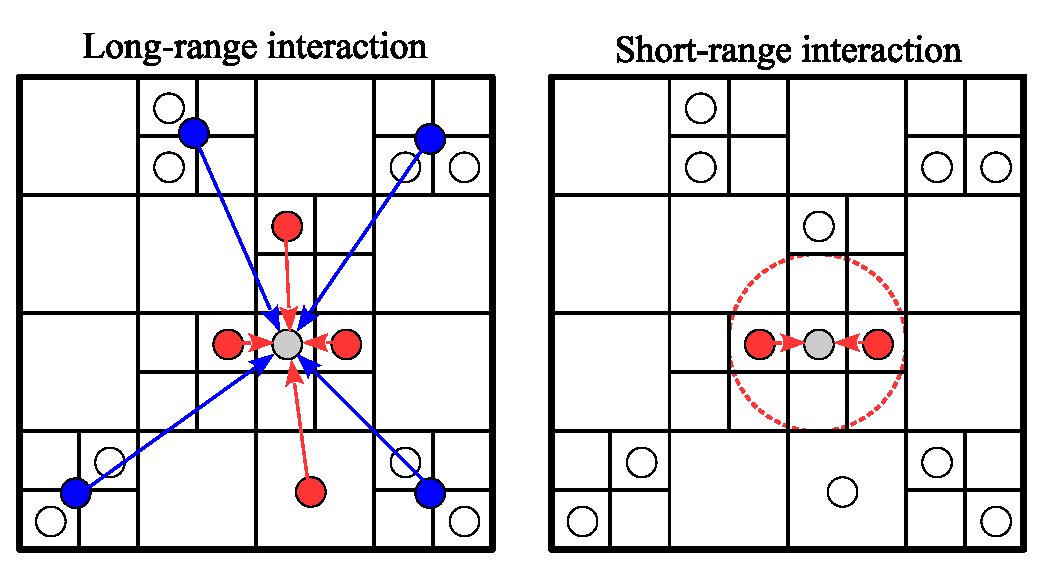
\includegraphics[width=8cm]{force_type.eps}
%  \end{center}
%  \caption{長距離力と短距離力のイメージ図。}
%  \label{fig:force}
%\end{figure}

また、粒子間相互作用の計算において、ある粒子は自分のプロセス以外の粒子
とも相互作用する可能性があるため、FDPS では相互作用に寄与する$j$ 粒子
を通信して相互作用を計算するのに必要な粒子を全て自分のプロセスに集める
方法を採用している。この方法では短距離力の場合は近傍のプロセスと通信す
れば良い。長距離力の場合にはBarnes-Hut tree法を採用しているため、遠く
の計算領域のプロセスからは全ての粒子をもらってくる必要はなく粒子が作る
ポテンシャルの多重極展開の係数を通信すれば十分であり、FDPS もこの方法
を採用している\cite{2004PASJ...56..521M}。

%図\ref{fig:LET} はプロセス間でのj 粒子の通信を表したものである。
%\begin{figure}
%  \begin{center}
%    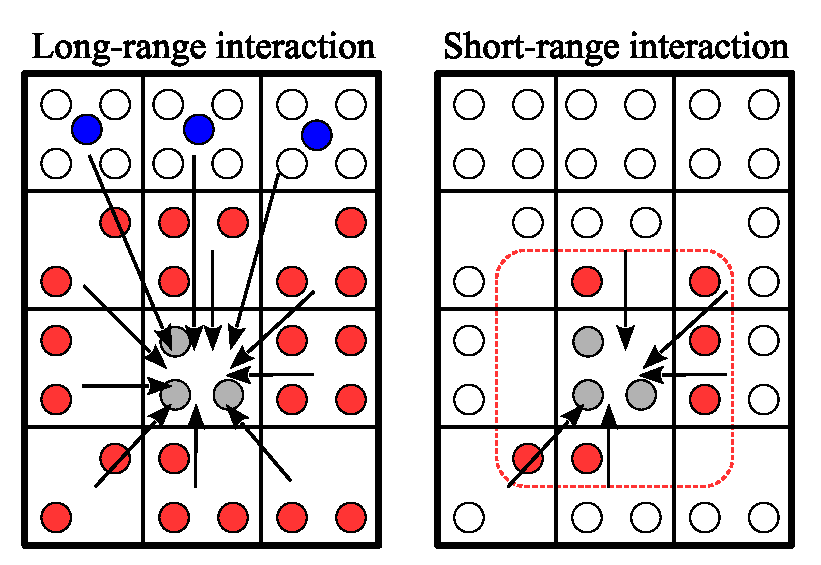
\includegraphics[width=8cm]{exchangeLET.eps}
%  \end{center}
%  \caption{長距離力と短距離力の場合のj粒子交換のイメージ図。}
%  \label{fig:LET}
%\end{figure}

ユーザーがこのクラスのメソッド{\tt
  TreeForForce::calcForceAllAndWriteBack()}を全てのプロセスで呼び出す
と、FDPSは粒子座標から木構造を構築し、相互作用の計算に必要な$j$粒子の
通信を行い、更に相互作用の計算までを行う。この関数内での木構造構築や相
互作用計算はOpenMPにも対応している。

複数種類の相互作用を計算する場合はこのクラスのオブジェクトを複数生成す
れば良い。


\section{PEZY-SC2 と Sunway Taihulight}

PEZY-SC2 の詳細をここで繰り返す必要はないが、1チップに 2048個 (そのうち
1984個を使用)のプロセッサを集積した MIMD アーキテクチャプロセッサであ
る。階層毎に共有範囲が広くなる3階層でコヒーレンシをもたない
データキャッシュと、プロセッサ毎に20KBのローカルメモリを持つ。この他に
チップ毎に6個の汎用のMIP64 コアが搭載されているが、我々が実装・評価を
行った時点ではこの MIPコアをプログラム実行に使うことはできず、
PCIe スイッチを経由して接続された Xeon-D プロセッサが16個の
PEZY-SC2 プロセッサを制御する。このため、Xeon-D プロセッサと
PEZY-SC2 プロセッサ1つの間の転送バンド幅は 1GB/s 程度と低くなり、
またホスト計算機も相対的に非力である。

Sunway Taihulight は史上初めて中国の独自開発のプロセッサとしてTop500リ
ストの1位、すなわち、HPLベンチマークの性能で世界一を達成したプロセッサ
である。1プロセッサチップは4つのコアグループからなり、それぞれのコアグ
ループは1つの制御プロセッサ(MPE)と64個の計算プロセッサ(CPE)から構成さ
れる。MPEとCPEはアーキテクチャは同じだが、MPE は通常のL1およびL2データ
キャッシュをもつのに対して、CPE はデータキャッシュをもたず、64KBのロー
カルメモリのみをもつ構成となっている。主記憶にはロード/ストア命令での
のアクセスの他、DMAコントローラによるローカルメモリとのデータ移動が可
能である。DMAコントローラは連続アクセスの他ストライドアクセスもでき、
また、比較短い転送長でもある程度の性能がでるように設計されている。さら
に、64個のコアは $8\times 8$ の2次元格子の構造をもち、縦・横方向の放送
や p2p 転送をレジスタ間で行うことができる。このため、CPE間は極めて低レ
イテンシ・高速な通信・同期が可能である。

プログラミングモデルは、SC2 は PZCL である。SW26010 は一応 OpenACC が
実装されているが使いものになるような性能はでない。Pthread ライブラリに
近いインターフェースをもつ Athread ライブラリというものを用いる。
Pthread と同様基本的に関数を起動するだけなので、プログラミングモデルと
しては比較的書きやすいものである。

コンパイラについては、SC2 はLLVMベースのモダンなコンパイラで、 4/8ス
レッドSMTであることもありある程度の最適化ができているが、SW26010 のコ
ンパイラはまだ極めて未熟なものであり、相互作用カーネル等についてはアセ
ンブラルーチンを記述する必要があった(イントリンシックやインラインアセ
ンブラの実装が十分なものでなかった)。

SW26010 と SC2 を比較すると、倍精度演算器の数は 1024 と2048で2倍違うが、
動作クロックも2倍違うためピーク性能は同程度、メモリバンド幅も同程度で
あり、非常に類似した特性をもっている。電力性能には大きな差があり、
SW26010のテクノロジーが不明だが、動作クロックが2倍違うことが大きな要因
と考えられる。SW26010 が4wayのSIMD プロセッサであることが電力性能の向
上にはあまり寄与していないように見えることは興味深い。


\section{FDPS の変更点}

FDPS のアクセラレータ向けの実装は存在しており、これは
GRAPE 向けのアルゴリズム\cite{Makino1991c} をGPGPU向けに
修正 \cite{Hamadaetal2009a}した multiwalk 法によるものである。
これは、相互作用計算のみをアクセスで行う、言い換えるとアクセラレータ
を相互作用専用計算機として使うものであり、実装は容易だが実現できる性能
には限界がある。重力計算以外の部分がホストプロセッサに残るため、
ホストプロセッサとアクセラレータの性能比があまり大きいと、アクセラレー
タの性能を有効に活用できない。

FDPS を利用した並列化粒子系シミュレーションコードは典型的には以下の手
順で計算を進める。

\begin{enumerate}

\item 領域分割を行う。ロードバランスを考慮してMPIプロセスが担当する領域の大きさを決める。
\item 各粒子を、それが存在する領域をもつMPIプロセスに移動する。
\item 各MPIプロセスが、自分の担当する粒子からツリー構造を作る。
\item 各MPIプロセスが、他の全プロセスに対して、それぞれが必要とする自
  分の情報(Local Essential Tree, LET)を構築し、MPI\_ALLTOALLV 関数で交
  換する
\item 各MPIプロセスが、もらった情報から系全体のツリー構造を作る
\item 相互作用計算を行う。全粒子を $n_g$ 個程度の粒子をもつグループに
  分け(これにもツリー構造をつかう)、それに対してツリーを辿って相互作用
  するセル・粒子のリスト(相互作用リスト)を構築する
\item 相互作用リストを使って相互作用計算をする
\item 計算した相互作用を使って粒子の時間積分を行う
\item 最初に戻る
\end{enumerate}

非常にプロセス数が多くても、「京」のようなアクセラレータをもたない計算
機ではこの手順で大きな問題はなかったが、アクセラレータやヘテロジニアス
アーキテクチャでは実際上全てのプロセスを見直す必要があった。
例えば領域分割では、ルートプロセスがサンプルした粒子から領域分割を構成
するサンプリングアルゴリズム\cite{BlackstonSuel1997}を使っていたが、
これはプロセス数 $p$のオーダーの処理がある。階層化した処理にすることで
$O(p^{1/3})$ の時間で処理できるアルゴリズムに変更した。次の、領域の変更や粒
子の移動に対応して粒子を送るところでは、従来 
MPI\_ALLTOALLV 関数を使っていたものを変更し、実際に送る範囲を同定して
その範囲で p2p 転送をするようにした。また、LET通信も
同様な工夫によってMPI\_ALLTOALLV 関数を排除した。
さらに、 ツリー構築等も CPE側や SC2側で実装した。さらに、
ツリー構築や相互作用リスト構築のコストを減らすため、1度作った相互作用
リストを複数ステップ使うアルゴリズム、分子動力学でいう bookkeeping
scheme をツリー法に拡張したものを実装した。

相互作用の計算は、SW26010ではアセンブラで実装した。SC2 でも十分な最適
化を行った。なお、 SC2 では半精度演算の利用もテストしたが、大きな高速
化は実現できていない。





\section{性能}

\begin{figure}
  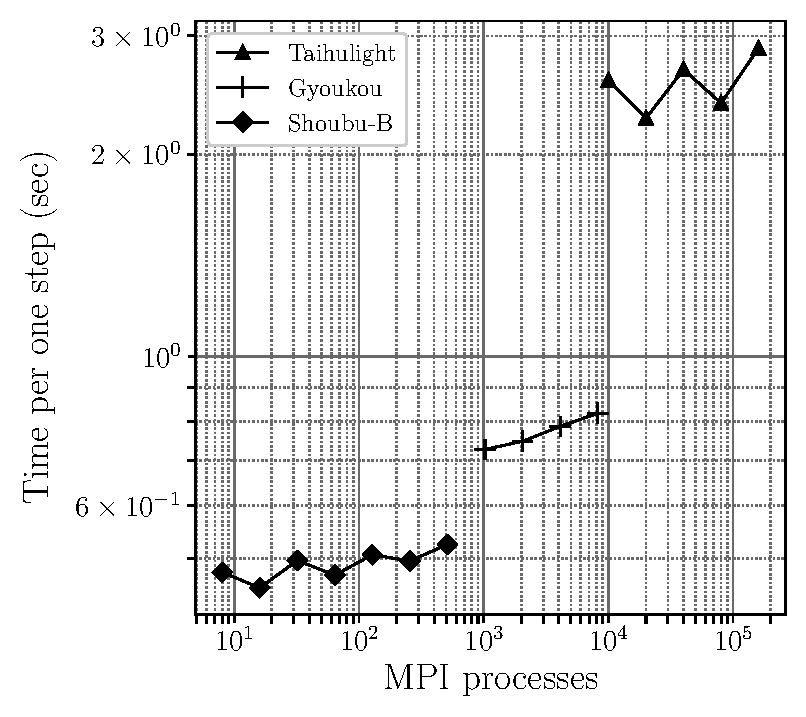
\includegraphics[width=8cm]{./weak_scaling2.eps}
  \caption{弱スケーリングテストでの1タイムステップあたりの性能。
    1MPIプロセスあたりの粒子数は $10^7$ である。三角、クロス、四角は
    Taihulight、暁光、菖蒲システムBでの計算時間をしめす。
  }
  \label{fig:weak}
\end{figure}

\begin{figure}
  \centering
  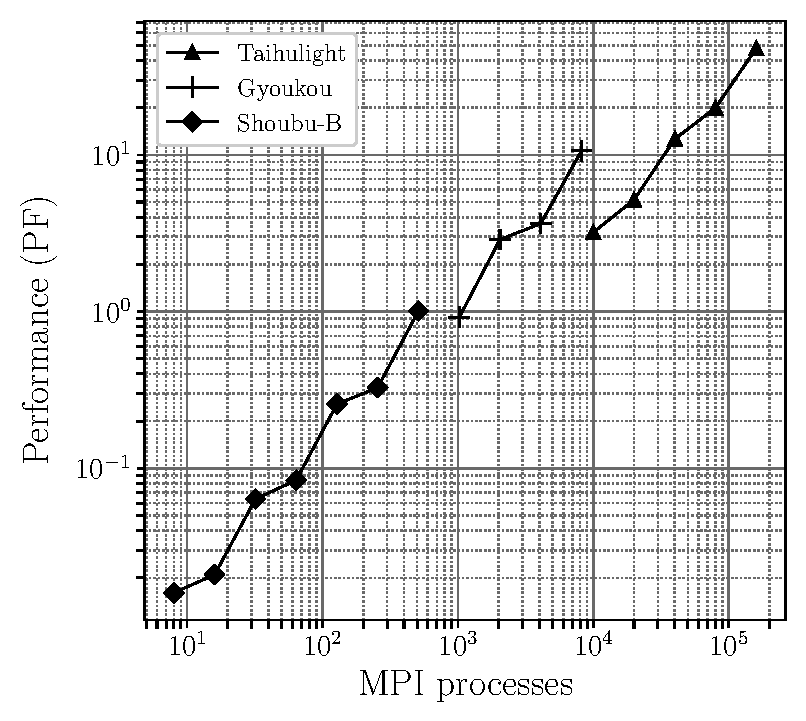
\includegraphics[width=8cm, clip]{./weak_scaling_speed.eps}
  \caption{図 \ref{fig:weak} と同じだがペタフロップス単位の計算速度をしめす。}
  \label{fig:weakpf}
\end{figure}

\begin{figure}
  \centering
  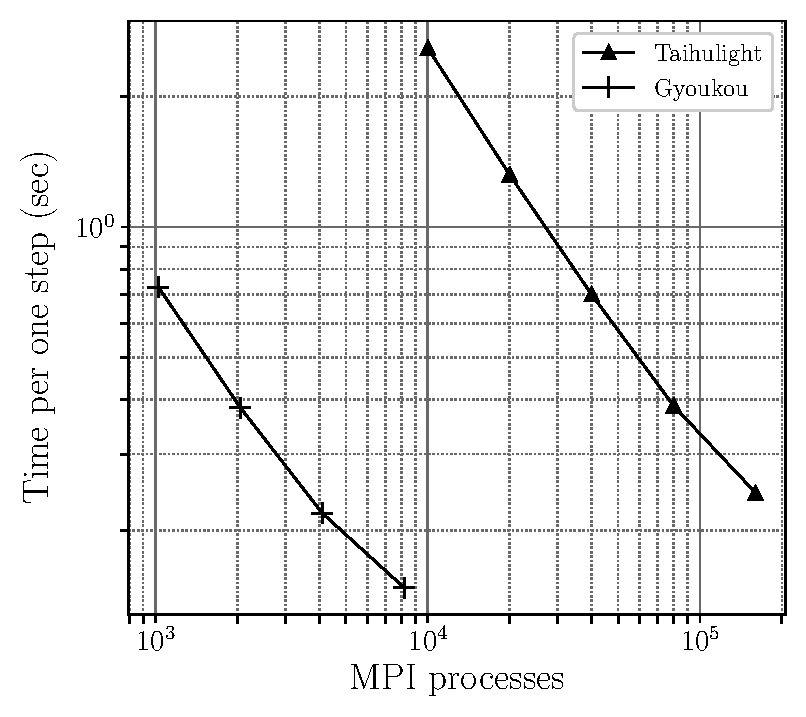
\includegraphics[width=8cm, clip]{./strong_scaling.eps}
  \caption{図 \ref{fig:weak} と同じだが強スケーリングでの計算時間をし
    めす。
    粒子数は Taihulight で $10^{11}$、SC2ベースのシステムでは $10^{10}$ である。}
  \label{fig:strong}
\end{figure}

図 \ref{fig:weak}と\ref{fig:weakpf} に弱スケーリングでの1ステッ
プあたりの時間と計算速度、図 \ref{fig:strong}に強スケーリングでの
1ステップあたり計算時間をしめす。対象とする問題は土星リングであり、
粒子間には重力の他物理的に衝突した時の反発力と、非弾性衝突を実現するた
めの抵抗力が働く。

測定は Sunway Taihulight (SW26010 フルシステム4万ノード)、暁光(SC2 フルシステム1万ノード)、菖蒲システムB(SC2 フルシステム512ノード)で行った。

図 \ref{fig:weak}から、弱スケーリング性能は極めて良好であることがわか
る。3システムの全てで、プロセス数を10倍以上変化させても、速度低下は
10\%程度である。同一のプロセッサである菖蒲システムBと暁光で性能に差が
あるが、これは暁光の運用が 2018/3/31 をもって停止されたために十分な最
適化ができなかったためである。菖蒲システムBでの最適化はこのあとも継続
した。

Taihulight 最大構成での性能は 47.9 PF であり、理論ピーク性能の 39.7\%
である。一方、暁光では 8192プロセッサで 10.6PF、理論ピークの 23.3\%、
菖蒲システムBでは512プロセッサで 1.01PF、 理論ピークの 35.5\%である。
但し、単精度演算をもたない Taihulight では相互作用計算が全て倍精度で行
われるが、SC2 では粒子座標等は倍精度だが相互作用計算のカーネル部分は
単精度で行われる。従って、ピーク性能に対する割合も単精度ピークでの値と
している。相互作用計算以外は全て倍精度で行われるため、相互作用計算が
高速になった結果ピークに対する効率が若干さがっており、ピーク性能からの
比率の SW26010とSC2の差はアーキテクチャの優劣をあらわすものではない。

但し、SC2 では逆数平方根関数ユニットのスループットが低いことが全体の効
率を落としていることは否定できない。多くの最近のプロセッサのように逆数
平方根の近似値を高いスループットでだすユニットと、ニュートン法等の反復
による精度向上を組合せたほうが実行効率はあげやすい。


\section{まとめと議論}



我々は大規模並列粒子法シミュレーションプログラム開発を容易にするフレー
ムワークFDPSをベースに、SC2 および同様なヘテロジニアスメニーコアアーキ
テクチャである SW26010 で高い効率をだすシミュレーションコードの開発を
おこなった。基本的なコンセプトを変更することなく、理論ピークの 35-40\%
という非常に高い効率を実現できた。ヘテロジニアスアーキテクチャの有効利
用に対するフレームワークによるアプローチの有効性を実証できたと考えてい
る。

2つのシステムでの実装の最適化をおこなった実感としては、正直なところ、
SW26010のほうが最適化は容易であったといえる。これは、

\begin{enumerate}

  \item 真のヘテロジニアスメニーコアアーキテクチャであり、MPEで動いて
    いるコードを少しづつ CPE に移動していくことでチューニング作業を進めることができた。
    
  \item キャッシュがない代わりにローカルメモリとDMA、コア間高速通信が
    あり、全て陽的に制御できるために実装の性能予測が容易である。このた
    め、色々やってみて性能が上がるかどうかテスト、というトライアルアン
    ドエラーの繰り返しがあまり多くなく、机上の検討が有効である。
    また、プロセッサ間のデータ共有が明示的な放送によって行えるため、
    共有キャッシュを繰り返しアクセスする必要がなく、オーバーヘッド
    が小さい
   
\end{enumerate}

というのが主な要因になる。MIMDプロセッサで共有キャッシュがあることは、
プログラミングが容易であるような印象を与えることに寄与
することは実証されているが、しかし、それが本当に
プログラミングを容易にしているかどうかは疑わしい。


\section*{謝辞}

SC2 での実装の大部分をおこなった PEZY Computing の坂本氏、中村氏(当時)、
木村氏に深く感謝いたします。

\bibliographystyle{plain}
 
\bibliography{/usr2/makino/papers/bibtex/allrefs.bib,ms}

\end{document}
